\documentclass[main]{subfiles}

\begin{document}

\section{Лекция 6}

Неформально пояснить, что такое поднятие, можно следующим образом: отображение <<наматывает>> свое поднятие на
окружность с помощью накрытия $ p $.

\begin{figure}[H]
	\centering 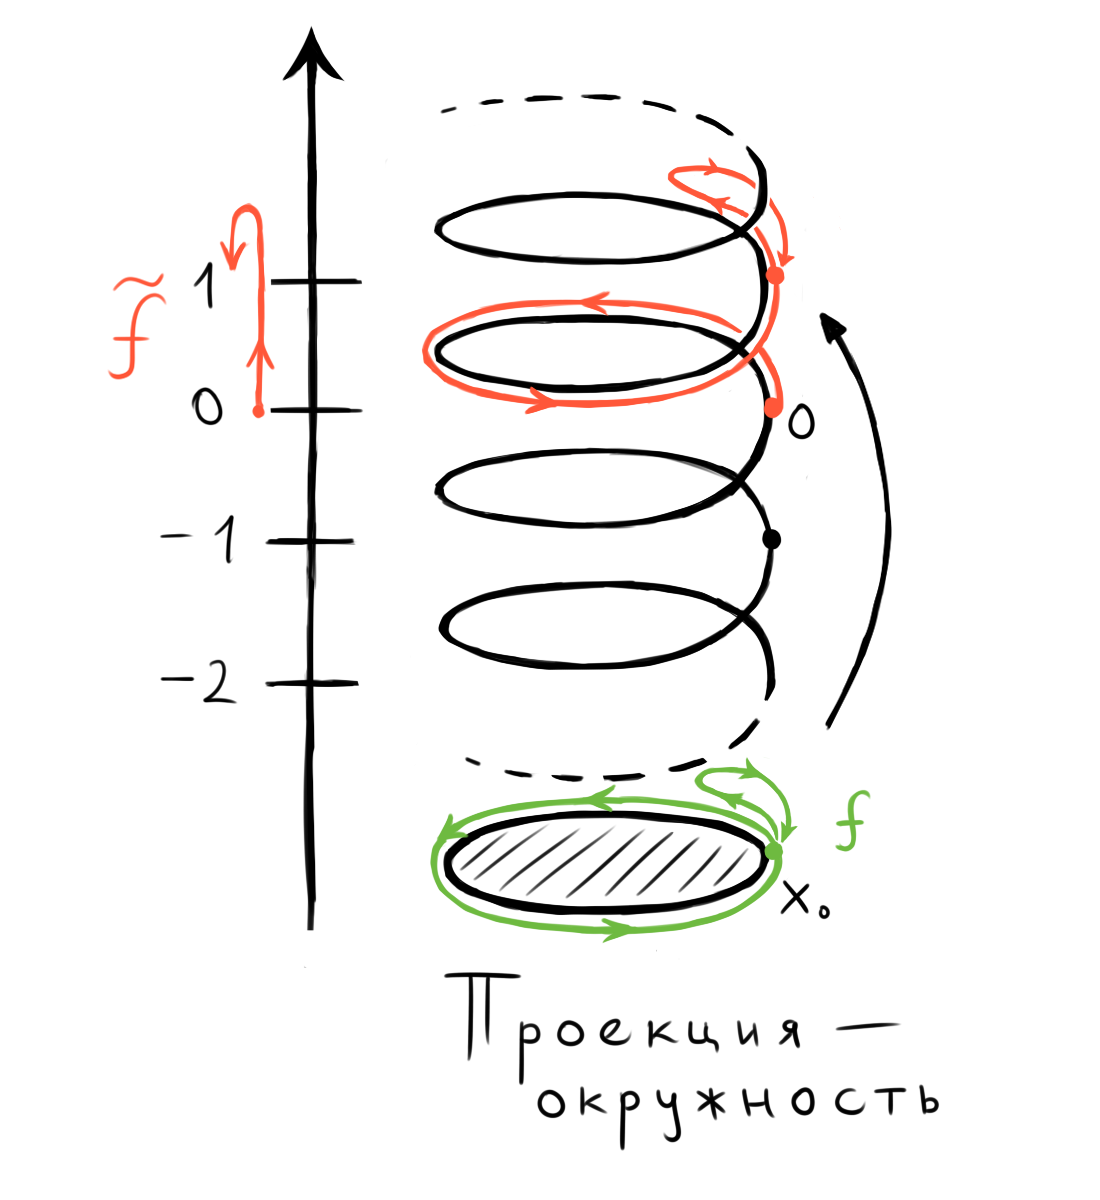
\includegraphics[width=0.5\textwidth]{lifting}
\end{figure}

\LiftExists

\begin{proof}
	Для всего отрезка $ [0; 1] $ мы не можем узнать, сколько целых окружностей всего пройдено, мы в
	точке знаем лишь дробную часть по модулю $ 2 \pi $. Однако если разбивать отрезок на малые
	части, то тогда можно считать, что на каждом кусочке была пройдена только соответствущая дробная часть;
	ни одного обхода окружности целиком.
	\begin{phased}
		\item[Существование.]
			Заметим, что если $ \Abs{z} = 1 $, то
			$ e^{2 \pi i \frac{\arg z}{2 \pi}} = \cos \arg z + i \sin \arg z = z $. Тогда можно положить
			$ \Up{f}(t) = \frac{1}{2 \pi} \arg f(t) $, однако в этом случае отображение не будет непрерывным.
			Поэтому положим $ \Up{f}(t) = \frac{1}{2 \pi} \arg f(t) + m(t) $, где $ m(t) \in \Z $, --- неформально,
			количество полных окружностей, пройденных путем $ f $ в точке $ t $, --- и оно будет непрерывным.

			Так как отображение $ f $ непрерывно на отрезке, то оно равномерно непрерывно на
			отрезке (то есть для любого $ \Eps > 0 $ существует такое $ \delta_\Eps > 0 $, что для любых
			$ t_1, t_2 \in [0; 1] $ если $ \Abs{t_1 - t_2} < \delta_\Eps $, то $ \Abs{f(t_1) - f(t_2)} < \Eps $).
			Рассмотрим такое число $ n \in \N $, что $ \frac{1}{n} < \delta_1 $.

			Для каждого
			$ k \in \Set{0, \ldots, n - 1} $ определим отображение
			$ h_k \colon \left[ \frac{k}{n}; \frac{k+1}{n} \right] \to \R $ следующим образом: для
			$ t \in \left[ \frac{k}{n}; \frac{k+1}{n} \right] $ положим
				$ h_k(t) = \arg \frac{f(t)}{f \left( \frac{k}{n} \right)}
				\in \left[ -\frac{\pi}{3}; \frac{\pi}{3} \right] $.
			Это отображение корректно определено (на окружности все точки не равны 0) и непрерывно,
			так как является разностью двух непрерывных функций (аргумент непрерывен, так как вся облать определения
			по одну сторону от точки 0). Аргумент в отрезке $ \left[ -\frac{\pi}{3}; \frac{\pi}{3} \right] $, так как
			расстояние между $ f(t) $ и $ f \left( \frac{k}{n} \right) $ меньше $ 1 $.

			Определим поднятие $ \Up{f} $ следующим образом: для каждого $ k \in \Set{0, \ldots, n - 1} $ и для
			любого $ t \in \left[ \frac{k}{n}; \frac{k + 1}{n} \right] $ положим
			\begin{dmath*}
				\Up{f}(t) =
				{ \frac{1}{2 \pi} \left( h_k(t) + \sum_{j = 0}^{k-1} h_j \left( \frac{j+1}{n} \right) \right) = }
				= {  \frac{1}{2 \pi} \left( \arg f(t) - \arg f \left( \frac{k}{n} \right) +
					\sum_{j = 0}^{k-1} \left(  \arg f \left(\frac{j+1}{n} \right) -
						\arg f \left( \frac{j}{n} \right) \right)
					+ 2 \pi m(t) \right) = }
				= {  \frac{1}{2 \pi } \arg f(t) + m(t) },
			\end{dmath*}
			где $ m(t) \in \Z $ --- некоторое целое число, зависящее от $ t $, которое появляется в силу того,
			что для любых $ z_1, z_2 \in \S^1 $
			верно $ \arg \frac{z_1}{z_2} = \arg z_1 - \arg z_2 + 2 \pi k $, $ k \in \Set{-1, 0, 1} $.

			Ясно, что отображение $ \Up{f} $ корректно определено, так как в точках вида $ \frac{k + 1}{n} $ выполнено
			равенство
				$ h_{k + 1} \left( \frac{k + 1}{n} \right) + \sum_{j = 0}^{k} h_j \left( \frac{j + 1}{n} \right)
				= 0 + h_k \left( \frac{k+1}{n} \right) + \sum_{j = 0}^{k-1} h_j \left( \frac{j + 1}{n} \right) $.
			Оно непрерывно, так как
			на каждом отрезке вида $ \left[ \frac{k}{n}; \frac{k + 1}{n} \right] $ является композицией непрерывных
			функций. Более того, ясно, что $ f = p \circ \Up{f} $. Таким образом, мы построили поднятие пути
			на окружности.
		\item[Единственность.] Пусть $ \Up{f}_1 $, $ \Up{f}_2$ --- два поднятия. Так как
			$ p \circ \Up{f}_1 = p \circ \Up{f}_2 $, то для любого $ t \in [0; 1] $ верно
			$ \Up{f}_1(t) - \Up{f}_2(t) \in \Z $. Так как поднятие непрерывны, то их разность тоже непрерывна,
			а значит, является константой. Так как $ \Up{f}_1(0) = \Up{f}_2(0) = 0 $, то оба поднятия совпадают.
	\end{phased}
\end{proof}

\begin{lemma} \label{lem.6.1}
	Две петли $ \phi_1 $, $ \phi_2 $ гомотопны $\iaoi$ их индексы равны.
\end{lemma}

\begin{proof} \leavevmode
	\begin{multiproof}
		\item[$\Then$] Раз петли гомотопны, то для каждого числа $ t \in [0; 1] $ существует непрерывное отображение
			$ f_t \colon ([0; 1], \Set{0, 1}) \to (\S^1, \Set{0})$, причем $ f_0 = \phi_1 $ и $ f_1 = \phi_2 $. Для
			этих отображений существуют поднятия $ \Up{f_t} $. Определим отображение $ h \colon [0; 1] \to \Z $:
			для $ t \in [0; 1] $ положим $ h(t) = \Up{f_t}(1) $. Без доказательства воспользуемая непрерывностю
		 	отображения $ h $. Тогда, так как $ h $ целочисленная, то это константа, а значит,
			$ h(0) = \Ind(\phi_1) = \Ind(\phi_2) = h(1) $.
		\item[$\If$] Очевидно, что любые два непрерывных отображения из $ [0; 1] $ в $ \R $ гомотопны. Тогда поднятия
			$ \Up{\phi_1}, \Up{\phi_2} \colon ([0; 1], \Set{0}) \to (\R, \Set{0}) $ гомотопны. Обозначим через
			$ \Up{F} \colon [0; 1]^2 \to \R $ эту гомотопию. Так как это гомотопия отображений пар, то тогда по
			определению для любого $ \tau \in [0; 1] $ выполнено $ \Up{F}(\Set{0}, \tau) \subseteq \Set{0} $, то есть
			$ \Up{F}(0, \tau) = 0 $. Положим $ F = p \circ \Up{F} $ и докажем, что это гомотопия петель $ \phi_1 $
			и $ \phi_2 $. Действительно, оно непрерывно как композиция непрерывных отображений, значения функции
			остаются во множестве $ \S^1 $, $ f_0 = \phi_1 $ и $ f_1 = \phi_2 $. Так как это гомотопия отображений
			пар, то также требуется проверить, что для любого $ \tau \in [0; 1] $ выполнено
			$ F(\Set{0, 1}, \tau) = \Set{0} $. Это действительно так, поскольку при $ t = 0 $ имеем
			$ F(0, \tau) = e^{2 \pi i \Up{F}(0, \tau)} = 1 $, а при $ t = 1 $ ввиду $ \Up{\phi_1}(1) = \Up{\phi_2}(1) $
			получаем $ F(1, \tau) = e^{2 \pi i \Up{F}(1, \tau)} = e^{2 \pi i \Ind(\phi_1)} = 1 $.
	\end{multiproof}
\end{proof}

\begin{theorem} \label{the.6.1}
	Определим отображение $ \psi \colon \pi_1(\S^1, 0) \to \Z $ следующти образом: для любой петли $ \phi $ положим
	$ \psi([\phi]) = \Ind(\phi) $. Тогда $ \psi $ --- изоморфизм групп $\pi_1(\S^1, 0)$ и $\Z$.
\end{theorem}

\begin{lemma} \label{lem.6.2}
	Пусть $ \phi_1 $, $ \phi_2 $ --- две петли, тогда
		\[ \Up{\phi_1 \phi_2}(t) = \begin{cases}
				\Up{\phi_2}(2 t), & \text{если } t \in \left[ 0; \frac{1}{2} \right], \\
				\Up{\phi_2}(1) + \Up{\phi_1}(2 t - 1), & \text{если } t \in \left[ \frac{1}{2}; 1 \right].
			\end{cases}
		\]
\end{lemma}

\begin{proof}[Доказательство теоремы \ref{the.6.1}] \leavevmode
	\begin{phased}
		\item[Корректность.]
			Надо доказать, что если две петли в одном классе эквивалентности, то у них одинаковый индекс.
			Это напрямую следует из леммы \ref{lem.6.1}.
		\item[Гомоморфность.] Надо доказать, что индекс композиции двух петель равен сумме индексов. С учетом леммы
			имеем:
			\[ \Ind(\phi_1 \phi_2) = \Up{\phi_1 \phi_2}(1) = \Up{\phi_2}(1) + \Up{\phi_1}(1) =
				\Ind(\phi_1) + \Ind(\phi_2), \]
			что и требовалось.
		\item[Эпиморфность.] Надо доказать, что для любого $ k \in \Z $ существует петля индекса $ k $. Действительно,
			в качестве такой петли можно взять петлю $ f_k $.
		\item[Мономорфность.] Надо докахать, что если у двух петель одинаковый индекс, то они в одном классе
			эквивалентности. Это напрямую следует из леммы \ref{lem.6.1}.
	\end{phased}
\end{proof}

\begin{proof}[Доказательство леммы \ref{lem.6.2}]
	В точке $ t = \frac{1}{2} $ отображение определено корретно, так как по определению $ \Up{\phi_1}(0) = 0 $.
	Рассмотрим теперь композицию $ p $ и $ \Up{\phi_1 \phi_2} $:
		\[ (p \circ \Up{\phi_1 \phi_2})(t) = \begin{cases}
				(p(\Up{\phi_2}(2 t)) = \phi_2(2 t),
					& \text{если } t \in \left[ 0; \frac{1}{2} \right]; \\
				p(\Up{\phi_2}(1) + \Up{\phi_1}(2 t - 1)) = e^{ 2 \pi i \Ind(\phi_2)} \phi_1(2 t - 1) = \phi_1(2 t - 1),
					& \text{если } t \in \left[ \frac{1}{2}; 1 \right],
			\end{cases}
		\]
	что и требовалось доказать.
\end{proof}

\end{document}
